\documentclass[a4paper,12pt]{article}
\usepackage{standalone}
\usepackage{amsmath} % Package for advanced math typesetting



% Basic
\usepackage[T1]{fontenc}
\usepackage[utf8]{inputenc}
\usepackage{titlesec}
\titleformat{\section}
  {\normalfont\fontsize{14}{15}\bfseries}{\thesection}{1em}{}
\titleformat{\subsection}
  {\normalfont\fontsize{12}{15}\bfseries}{\thesubsection}{1em}{}

% Changes sections from 1.1 to 1.a
\renewcommand{\thesubsection}{\thesection.\alph{subsection}}

% ------------------------------------------------------------ %

% Packages
\RequirePackage{tcolorbox}
\usepackage{amsmath, amsthm, amssymb}
\usepackage{blindtext}
\usepackage{enumitem}
\usepackage{extramarks}
\usepackage{fancyhdr}
\usepackage[margin=1in]{geometry}
\usepackage{graphicx}
\usepackage{hyperref}
\usepackage{indentfirst}
\usepackage{listings}
\usepackage{mathrsfs}
\usepackage{mdframed}
\usepackage{multicol, multirow}
\usepackage{needspace, setspace}
\usepackage{paracol}
\usepackage{pgf, pgfplots}
\usepackage{tikz}
\usetikzlibrary{patterns}
\usepackage{silence}
\usepackage{xcolor}
\usepackage{bookmark}
\setlength{\parindent}{0pt}
\usetikzlibrary{patterns}
% \usepackage{subcaption}
\usetikzlibrary{decorations.pathreplacing}
\usepackage{caption}
\usepackage{subcaption}
\usepackage{xcolor}
\definecolor{maroon}{RGB}{128, 0, 0}
% ------------------------------------------------------------ %

% Spacings
\newcommand{\n}{\vspace{3mm}} % Context spacing
\newcommand{\s}{\vspace{1mm}} % Equation spacing
\newcommand{\m}{\vspace{-3mm}} % Reverse context spacing
\newcommand{\propdisp}{\pagebreak} % Proper display page break
\newcommand{\br}{\n\\\n}

% Wordings
\newcommand{\ans}[1][zb]{{\color{#1}\textit{Answer. }\hspace{3mm}}} % Answer
\newcommand{\arl}[1][zr]{{\color{#1}$\brr{\Leftarrow}$\hspace{3mm}}} % Left arrow
\newcommand{\arr}[1][zr]{{\color{#1}$\brr{\Rightarrow}$\hspace{3mm}}} % Right arrow
\newcommand{\cse}[2][zr]{{\color{#1}\textit{Case #2: }\hspace{1mm}}} % Case
\newcommand{\clm}[2][zr]{{\color{#1}$\vdash_{#2}$\hspace{1mm}}} % Claim
\newcommand{\prf}[1][zr]{{\color{#1}\textit{Proof. }\hspace{3mm}}} % Proof
\newcommand{\prt}[2][a]{\hspace{-2mm}{\color{#2}\textit{Part (#1) }}\hspace{1mm}} % Part
\newcommand{\prtc}[2][a]{\hspace{2mm}\prt[#1]{#2}} % Continued part

\newcommand{\rdft}[1][\sct]{{\color{zg}\textit{Definition #1}}} % Refer definition
\newcommand{\rexm}[1][\sct]{{\color{zb}\textit{Example #1}}} % Refer example
\newcommand{\rfig}[1][\sct]{{\color{zy}\textit{Figure #1}}} % Refer figure
\newcommand{\rpst}[1][\sct]{{\color{zr}\textit{Proposition #1}}} % Refer proposition
\newcommand{\rthm}[1][\sct]{{\color{zr}\textit{Theorem #1}}} % Refer theorem

\newcommand{\sct}{\thesection.\thescount} % Counter
\newcommand{\sctr}[2][0]{\the\numexpr\value{section}-#1\relax.\the\numexpr\value{scount}-#2\relax} % Relative counter

% Equations
\newcommand{\C}{\mathbb{C}} % Complex
\newcommand{\F}{\mathbb{F}} % Field
\newcommand{\I}{\mathbb{I}} % Irrational
\newcommand{\N}{\mathbb{N}} % Natural
\newcommand{\Q}{\mathbb{Q}} % Rational
\newcommand{\R}{\mathbb{R}} % Real
\newcommand{\Z}{\mathbb{Z}} % Integer

\newcommand{\GL}{\mathrm{GL}} % General linear group
\newcommand{\SL}{\mathrm{SL}} % Special linear group

\newcommand{\abs}[1]{\left| #1\right|} % Absolute
\newcommand{\bra}[1]{\left\langle #1\right\rangle} % Angled brackets
\newcommand{\brc}[1]{\left\{ #1\right\}} % Curly brackets
\newcommand{\brr}[1]{\left( #1\right)} % Round brackets
\newcommand{\brs}[1]{\left[ #1\right]} % Square brackets
\newcommand{\cond}[1]{\left. #1\right|} % Condition with right bar
\newcommand{\diff}{\,\mathrm{d}} % Differential
\newcommand{\erm}[1]{\;\;\;\;\text{#1}} % Equation remarks
\newcommand{\nrm}[1]{\left\| #1\right\|} % Norm
\newcommand{\srm}{\,\mid\,} % Set remarks

% Math operators
\let\Im\relax
\let\Re\relax

\DeclareMathOperator{\Im}{Im} % Imaginary function
\DeclareMathOperator{\Re}{Re} % Real function

% ------------------------------------------------------------ %

% Colours
\definecolor{gr}{RGB}{120, 120, 120} % Grey
\definecolor{zb}{RGB}{0, 38, 77} % Blue
\definecolor{zg}{RGB}{0, 77, 51} % Green
\definecolor{zp}{RGB}{51, 0, 77} % Purple
\definecolor{zr}{RGB}{77, 0, 38} % Red
\definecolor{zy}{RGB}{77, 64, 0} % Yellow

% Graphing
\usetikzlibrary{arrows}
\usetikzlibrary{calc}
\usetikzlibrary{patterns}
\pgfplotsset{compat=1.15}

% ------------------------------------------------------------ %

% Remark
\newcommand{\remark}[1]{
  \noindent\textbf{Remarks}
  
  \begin{nlist}
    \item Context of this document is based on university course \textit{\gettitle} from \textit{Department of Mathematics, The Chinese University of Hong Kong}. The original source can be found at \url{https://www.math.cuhk.edu.hk/course}. The author does not own the source.
    \item This document is assumed unavailable for unauthorized parties that have not attended the university course. It is prohibited to share, including distributing or copying this document to unauthorized parties in any means for any non-academic purpose.
    \item Context of this doucment may not be completely accurate. The author assumes no responsibility or liability for any errors or omissions in the context of this document.
    \item This document is under license CC-BY-SA 4.0. It is allowed to make any editions on this document, as long as terms of the license is not violated.
    #1
  \end{nlist}
}

% Prerequisites
\newenvironment{prereq}{
  \noindent \textbf{Prerequisites}\n

  This course requires prerequisites of
}{
  \n
}

% Reference list
\newenvironment{reflist}{
  \begin{alist}
    \item Course material from various professors associated to \textit{\gettitle}
}{
  \end{alist}
}

% ------------------------------------------------------------ %

% Environments
\newcounter{scount}[section] % Counter

\newenvironment{crl}{ % Corollary
  \parindent 0pt
  \begin{siderule}[linecolor=zr]{\color{zr}\textit{Corollary. }}
}{
  \end{siderule}
}

\newenvironment{cmt}{ % Comment
  \parindent 0pt
  \begin{siderule}[linecolor=zp]{\color{zp}\textit{Comment. }}
}{
  \end{siderule}
}

\newenvironment{dft}{ % Definition
  \parindent 0pt
  \refstepcounter{scount}
  \begin{siderule}[linecolor=zg]{\color{zg}\textit{Definition \sct. }}
}{
  \end{siderule}
}
\newenvironment{lem}{ % Lemma
  \parindent 0pt
  \refstepcounter{scount}
  \begin{siderule}[linecolor=zg]{\color{zg}\textit{Lemma \sct. }}
}{
  \end{siderule}
}

\newenvironment{exm}{ % Example
  \parindent 0pt
  \refstepcounter{scount}
  \begin{siderule}[linecolor=zb]{\color{zb}\textit{Example \sct. }}
}{
  \end{siderule}
}

\newenvironment{fig}{ % Figure
  \parindent 0pt
  \refstepcounter{scount}
  \begin{siderule}[linecolor=zy]{\color{zy}\textit{Figure \sct. }}\n
  
}{
  \end{siderule}
}

\newenvironment{prv}{ % Proof
  \parindent 0pt
  \begin{siderule}[linecolor=zr]\prf
}{
  \end{siderule}
}

\newenvironment{pst}{ % Proposition
  \parindent 0pt
  \refstepcounter{scount}
  \begin{siderule}[linecolor=zr]{\color{zr}\textit{Proposition \sct. }}
}{
  \end{siderule}
}

\newenvironment{tcn}{ % Technique
  \parindent 0pt
  \begin{siderule}[linecolor=zp]{\color{zp}\textit{Technique. }}
}{
  \end{siderule}
}

\newenvironment{thm}{ % Theorem
  \parindent 0pt
  \refstepcounter{scount}
  \begin{siderule}[linecolor=zr]{\color{zr}\textit{Sætning \sct. }}
}{
  \end{siderule}
}

\newenvironment{rmatrix}{ % Matrix in round brackets
  \left(\begin{matrix}
}{
  \end{matrix}\right)
}

\newenvironment{alist}{ % Alphabetical list
  \begin{enumerate}[label=(\alph*)]
}{
  \end{enumerate}
}

\newenvironment{Alist}{ % Capitalized alphabetical list
  \begin{enumerate}[label=(\Alph*)]
}{
  \end{enumerate}
}

\newenvironment{nlist}{ % Number list
  \begin{enumerate}[label=(\arabic*)]
}{
  \end{enumerate}
}

\newenvironment{plist}{ % Point list
  \begin{itemize}
}{
  \end{itemize}
}

\newenvironment{rlist}{ % Roman list
  \begin{enumerate}[label=(\roman*)]
}{
  \end{enumerate}
}

\newmdenv[ % Siderule line
  topline=false,
  bottomline=false,
  rightline=false,
  rightmargin=0
]{siderule}


% ------------------------------------------------------------ %
% Warning filters
\WarningFilter{mdframed}{You got a bad break}
\hfuzz=8pt


% Load required packages
\usepackage{tcolorbox}
% ------------------------------------------------------------ %

% Code

\usepackage{amsmath}
\usepackage{graphicx}
\definecolor{bluekeywords}{rgb}{0.13,0.13,1}
\definecolor{greencomments}{rgb}{0,0.5,0}
\definecolor{redstrings}{rgb}{0.9,0,0}
\definecolor{bgcolor}{rgb}{0.95,0.94,0.94}
\usepackage{listings}
\usepackage{upquote}
\usepackage{xcolor}

\lstdefinelanguage{Python}
{
  keywords={typeof, null, catch, switch, in, int, str, float, self},
  keywordstyle=\color{ForestGreen}\bfseries,
  ndkeywords={boolean, throw, import},
  ndkeywords={return, class, if ,elif, endif, while, do, else, True, False , catch, def},
  ndkeywordstyle=\color{BrickRed}\bfseries,
  identifierstyle=\color{black},
  sensitive=false,
  comment=[l]{\#},
  morecomment=[s]{/*}{*/},
  commentstyle=\color{purple}\ttfamily,
  stringstyle=\color{red}\ttfamily,
}

\lstset
{ %Formatting for code in appendix
    language=Python,
    numbers=left,
    stepnumber=1,
    showstringspaces=false,
    tabsize=1,
    breaklines=true,
    breakatwhitespace=false,
    backgroundcolor=\color{bgcolor},  % Background color
    basicstyle=\ttfamily\footnotesize, % Code font size and style
    frame=single,                    % Adds a frame around the code
    rulecolor=\color{bgcolor},       % Frame color
    breaklines=true,                 % Breaks long lines
}
 % Assuming these files exist and are correctly referenced
\graphicspath{ {../../pictures/IDMA/IDMA3_a}} % Assuming a pictures folder has been made and is correctly referenced

% \renewcommand{\thesection}{5.\arabic{section}} % Substitue 5. for any number

% Changes sections from 1.1 to 1.a
\renewcommand{\thesubsection}{\thesection.\alph{subsection}}

\begin{document}
% \includepdf[pages=-]{../../pictures/forside}

\title{Københavns Universitet\\
Introduktion til diskret matematik og algoritmer - Problem set 3}
\author{Victor Vangkilde Jørgensen}
\makeatletter
\let\getauthor\@author
\let\gettitle\@title
\makeatother
\maketitle
\thispagestyle{empty}
\n\n
 % Assuming this file contains the cover page setup

\pagebreak
\pagestyle{empty}
\tableofcontents
\pagebreak
\pagestyle{fancy}
\fancyhf{}
\setlength{\headheight}{15.2pt}
\renewcommand{\footrulewidth}{0.4pt}
% \fancyhead[R]{\nouppercase \lastrightmark}
\fancyfoot[L]{\gettitle}
\fancyfoot[R]{\thepage}
 % Assuming this file contains the header setup
\maketitle % This command will actually insert the title into the document


\section[Question 1]{Recall that a standard deck of cards has $52$ cards partitioned into four suits (hearts,
spades, clubs, and diamonds) with $13$ ranks each (2-10 plus jack, queen, king, and ace). In this
problem, we assume that you are dealt $5$ cards from a perfectly shuffled deck of cards.}

\subsection[]{What is the probability that you get a flush, i.e., $5$ cards of the same suit but not all in
sequence with respect to rank? (Because five cards of the same suit in sequential rank
would be a straight flush.)}

Først skal vi finde ud af, hvor mange mulige hænder vi kan trække. Siden vi får 5 tilfældige kort uden tilbagelægning, og rækkefølgen ikke betyder noget, kan vi beskrive dette som en binomialkoefficient:
\[ _{52}C_5 = {52 \choose 5} =\]
\[\dfrac{52!}{(52-5)! \cdot 5!} =\]
\[\dfrac{52!}{47! \cdot 5!} = 2.598.960\]
Nu skal vi bestemme mængden af hænder, der laver en flush. Der er 4 forskellige kulører, og vi skal bruge 5 af samme kulør:
\[ _{13}C_5 = {13 \choose 5} = \]
\[ \dfrac{13!}{(13-5)! \cdot 5!} = \]
\[ \dfrac{13!}{8! \cdot 5!} = 1287 \]
Vi skal dog også huske, at der er 4 forskellige kulører, så vi vælger 1 af de 4:
\[ _4C_1 \cdot 1287 = {4 \choose 1} \cdot 1287 = \]
\[ \dfrac{4!}{(4-1)! \cdot 1!} \cdot 1287 = \]
\[ \dfrac{4!}{3!} \cdot 1287 = \]
\[ 4 \cdot 1287 = 5148\]
Der er dog også mulighed for at trække en straight flush, som vi skal trække fra:
\[ _{10}C_1 \cdot _4C1 = {10 \choose 1} \cdot {4 \choose 1} = \]
\[ \dfrac{10!}{(10-1)! \cdot 1!} \cdot \dfrac{4!}{(4-1)! \cdot 1!} = \]
\[ \dfrac{10!}{9!} \cdot \dfrac{4!}{3!} = \]
\[ 10 \cdot 4 = 40\]
Så den samlede mængde af hænder, der laver en flush uden en straight flush, er:
\[ 5148 - 40 = 5108\]
Så sandsynligheden for at trække en flush er:
\[ \dfrac{5108}{2598960} \approx 0.00197\]

\subsection[]{What is the probability that you get a straight, i.e., $5$ 
cards of sequential rank but not all of the same suit? (Because if the latter condition also held, 
we would again have a straight flush.)
}

Vi bestemmer mængden af hænder, der laver en straight. Den laveste straight vi kan lave er $A, 2, 3, 4, 5$, og den højeste er $10, J, Q, K, A$. Fra $A$ til 10 er der 10 måder at lave en straight, hvis vi bare tæller fra og med laveste kort tal af straight'en op til de 10.
\[ _{10}C_1 = {10 \choose 1} = \]
\[ \dfrac{10!}{(10-1)! \cdot 5!} = \]
\[ \dfrac{10!}{9! \cdot 1!} = 10 \]
Vi skal dog også huske, at der er 4 forskellige kulører, så vi vælger 1 af de 4, for hvert af de 5 kort.
\[ _4C_1 \cdot _4C_1 \cdot _4C_1 \cdot _4C_1 \cdot _4C_1 \cdot 10 = {4 \choose 1} \cdot {4 \choose 1} \cdot {4 \choose 1} \cdot {4 \choose 1} \cdot {4 \choose 1} \cdot 10 = \]
\[ \dfrac{4!}{(4-1)! \cdot 1!} \cdot \dfrac{4!}{(4-1)! \cdot 1!} \cdot \dfrac{4!}{(4-1)! \cdot 1!} \cdot \dfrac{4!}{(4-1)! \cdot 1!} \cdot \dfrac{4!}{(4-1)! \cdot 1!} \cdot  10 = \]
\[ \dfrac{4!}{3!} \cdot \dfrac{4!}{3!} \cdot \dfrac{4!}{3!} \cdot \dfrac{4!}{3!} \cdot \dfrac{4!}{3!} \cdot 10 = \]
\[ 4 \cdot 4 \cdot 4 \cdot 4 \cdot 4 \cdot 10 = 10240\]
Der er dog også mulighed for at trække en straight flush, som vi skal trække fra:
\[ 10240 - 40 = 10200\]
Så sandsynligheden for at trække en straight er:
\[ \dfrac{10200}{2598960} \approx 0.00393\]


\section[Question 2]{Prove mathematically that among all numbers on the form $11...100...0$, i.e., numbers
consisting of $m$ ones followed by $n$ zeros for some $m,n \in N^+$ (sometimes notation like $1^m0^n$ is
used to describe text strings constructed in such a way), there is some number that is divisible
by 2025. Hint: Look at all numbers $1^m = 11 ... 1$ and consider what their remainders can be modulo $2025$.}

For at omformulere opgaven, skal vi vise:
\[ \exists m,n \in \N^+ \quad 2025 \mid 1^m0^n\]


\section[Question 3]{Let $a \in R^+$ be any positive real number. Show that for any integer $n \geq 2$ there is a
rational number $\frac{c}{d}, c,d \in \Z, d \leq n$, that approximates $a$ to within error $\frac{1}{dn}$, ie., $|a - \frac{c}{d}| \leq \frac{1}{dn}$.
Hint: Consider the numbers $a, 2a, \dots ,n \cdot a$ and show that one of these numbers is at distance at most $\frac{1}{n}$ from some integer.}



\section[Question 4]{In this problem we focus on relations. Suppose that $A = \{e_0,e_1,\dots,e_5\}$ is a set of
$6$ elements and consider the relation $R$ on $A$ represented by the matrix
\[M_R = 
    \begin{bmatrix}
        0 & 0 & 1 & 0 & 0 & 0 \\
        0 & 0 & 0 & 1 & 0 & 0 \\
        0 & 0 & 0 & 0 & 1 & 0 \\
        0 & 0 & 0 & 0 & 0 & 1 \\
        1 & 0 & 0 & 0 & 0 & 0 \\
        0 & 1 & 0 & 0 & 0 & 0 \\
    \end{bmatrix}
\]
(where element $e_i$ corresponds to the row and column $i+1$).}
\subsection[]{Let us write $S$ to denote the symmetric closure of the relation $R$. 
What is the matrix representation of $S$? Can you explain in words what the relation $S$ is by describing how it can be interpreted?
}

Vi får givet en matrice med relationen $R$ på $A$. Vi ser, at hvis vi repræsenterer matricen som en graf, ender vi med en directed graf, da alle vertices har en directed edge, og ingen af disse går tilbage igen. Grafisk er dette 2 'lukkede' cykler. Den symetriske closure af en matrix består af dens relation $R$ og dens converse relation $R^{-1}$. For en relation $R$ er dette defineret som: 
\[ R^{-1} = (b,a) : (a,b) \in R\]
som når anvendt på en matrix beskrives som:
\[M_{R^{-1}} = M_{R}^T = 
    \begin{bmatrix}
        0 & 0 & 0 & 0 & 1 & 0 \\
        0 & 0 & 0 & 0 & 0 & 1 \\
        1 & 0 & 0 & 0 & 0 & 0 \\
        0 & 1 & 0 & 0 & 0 & 0 \\
        0 & 0 & 1 & 0 & 0 & 0 \\
        0 & 0 & 0 & 1 & 0 & 0 \\
    \end{bmatrix}
\]

Vi bemærker, at dette er grafisk repræsenteret som de samme 2 lukkede cykler som før, dog er retningerne af edges'ne omvendt.

\[M_S = M_R \lor M_{R}^T = 
    \begin{bmatrix}
        0 & 0 & 1 & 0 & 0 & 0 \\
        0 & 0 & 0 & 1 & 0 & 0 \\
        0 & 0 & 0 & 0 & 1 & 0 \\
        0 & 0 & 0 & 0 & 0 & 1 \\
        1 & 0 & 0 & 0 & 0 & 0 \\
        0 & 1 & 0 & 0 & 0 & 0 \\
    \end{bmatrix}
    \lor
    \begin{bmatrix}
        0 & 0 & 0 & 0 & 1 & 0 \\
        0 & 0 & 0 & 0 & 0 & 1 \\
        1 & 0 & 0 & 0 & 0 & 0 \\
        0 & 1 & 0 & 0 & 0 & 0 \\
        0 & 0 & 1 & 0 & 0 & 0 \\
        0 & 0 & 0 & 1 & 0 & 0 \\
    \end{bmatrix}
    = 
    \begin{bmatrix}
        0 & 0 & 1 & 0 & 1 & 0 \\
        0 & 0 & 0 & 1 & 0 & 1 \\
        1 & 0 & 0 & 0 & 1 & 0 \\
        0 & 1 & 0 & 0 & 0 & 1 \\
        1 & 0 & 1 & 0 & 0 & 0 \\
        0 & 1 & 0 & 1 & 0 & 0 \\
    \end{bmatrix}
\]

Resultatet er, at de 2 lukkede cykler nu både har udgående edges fra $M_R$ og $M^T_{R}$. Edges'ne går nu bidirectional for alle edges i grafen, eksempelvis har $e_1$ en edge til $e_3$ i $M_R$, og $e_3$ har en edge til $e_1$ i $M^T_{R}$. Da dett gøres for alle edges, er grafen for $M_S$ bidirectional.

\subsection[]{Now let $T$ be the transitive closure of the relation $S$. What is the matrix representation of $T$? 
Can you explain in words what the relation $T$ is by describing how it can be interpreted?
}

Vi husker, at for en relation $R$ er dens transitive bestemt som: 
\[\brr{(a,b) \wedge (b,c)} \Rightarrow (a,c) : a,b,c \in R\]
For vores relation $S$ på matrix'en $M_S$ kan vi beskrive dette som:
\[M_T = M_S \lor M^2_S \lor M^3_S \lor \dots \lor M^n_S\]
eller
\[M_T =\bigvee \limits_{i=1}^{n} M^i_S\]
Rent sprogligt kan vi fortolke dette som at vi har alle de edges $M_T$, som er i $M_S$, og alle de edges, der kan nås fra $M_S$ i $n$ steps. Dette betyder, at hvis vi har en edge fra $e_1$ til $e_2$ i $M_S$, og en edge fra $e_2$ til $e_3$ i $M_S$, så vil der også være en edge fra $e_1$ til $e_3$ i $M_T$.\\
Vi kender i forvejen $M_S$, så vi går videre til $M^2_S$

\[M^2_S = M_S \lor M_S = 
\begin{bmatrix}
    0 & 0 & 1 & 0 & 1 & 0 \\
    0 & 0 & 0 & 1 & 0 & 1 \\
    1 & 0 & 0 & 0 & 1 & 0 \\
    0 & 1 & 0 & 0 & 0 & 1 \\
    1 & 0 & 1 & 0 & 0 & 0 \\
    0 & 1 & 0 & 1 & 0 & 0 \\
\end{bmatrix}
\lor
\begin{bmatrix}
    0 & 0 & 1 & 0 & 1 & 0 \\
    0 & 0 & 0 & 1 & 0 & 1 \\
    1 & 0 & 0 & 0 & 1 & 0 \\
    0 & 1 & 0 & 0 & 0 & 1 \\
    1 & 0 & 1 & 0 & 0 & 0 \\
    0 & 1 & 0 & 1 & 0 & 0 \\
\end{bmatrix}
=
\begin{bmatrix}
    1 & 0 & 1 & 0 & 1 & 0 \\
    0 & 1 & 0 & 1 & 0 & 1 \\
    1 & 0 & 1 & 0 & 1 & 0 \\
    0 & 1 & 0 & 1 & 0 & 1 \\
    1 & 0 & 1 & 0 & 1 & 0 \\
    0 & 1 & 0 & 1 & 0 & 1 \\
\end{bmatrix}\]

Når vi undersøger $M^2_S$, ser vi at elementer i cykel 1 ($e_0, e_2, e_4$) har 1 på positioner svarende til cykel 1, og elementer i cykel 2 ($e_1, e_3, e_5$) har 1 på positioner svarende til cykel 2. Der er altså 1 på hele diagonalen, hvilket betyder, at hvert element kan nå sig selv på 2 skridt i en cykel med 3 elementer. Vi kan verificere at $M^3_S = M^2_S$, hvilket betyder at vi har nået et fast punkt, og yderligere matrix potenser vil ikke ændre resultatet.

\[M_T = 
\begin{bmatrix}
    1 & 0 & 1 & 0 & 1 & 0 \\
    0 & 1 & 0 & 1 & 0 & 1 \\
    1 & 0 & 1 & 0 & 1 & 0 \\
    0 & 1 & 0 & 1 & 0 & 1 \\
    1 & 0 & 1 & 0 & 1 & 0 \\
    0 & 1 & 0 & 1 & 0 & 1 \\
\end{bmatrix}\]

Vi er nu færdige. Kort sagt kan vi fortolke grafen for $M_T$ som to bidirectional cykler baseret på om deres indeks er lige eller ulige, og hvor vertex danner en edge med sig selv.

\subsection[]{Suppose that we instead let $T^\prime$ be the transitive closure of the relation $R$, and then let
$S^\prime$ be the symmetric closure of $T^\prime$. Are $S^\prime$ and $T$ the same relation? If they are not the
same, show some way in which they differ. If they are the same, is it true that $S^\prime$ and $T$
constructed in this way from some relation $R$ on a set $A$ will always be the same? Please
make sure to motivate your answers clearly.
}

Vi udregner $R$ transitive closure på samme måde vi gjorde for $S$ tidligere. Vi kender $M_R$, så lad os udregne $M^2_R$:

\[M^2_R = M_R \lor M_R =
\begin{bmatrix}
    0 & 0 & 1 & 0 & 0 & 0 \\
    0 & 0 & 0 & 1 & 0 & 0 \\
    0 & 0 & 0 & 0 & 1 & 0 \\
    0 & 0 & 0 & 0 & 0 & 1 \\
    1 & 0 & 0 & 0 & 0 & 0 \\
    0 & 1 & 0 & 0 & 0 & 0 \\
\end{bmatrix}
\lor
\begin{bmatrix}
    0 & 0 & 1 & 0 & 0 & 0 \\
    0 & 0 & 0 & 1 & 0 & 0 \\
    0 & 0 & 0 & 0 & 1 & 0 \\
    0 & 0 & 0 & 0 & 0 & 1 \\
    1 & 0 & 0 & 0 & 0 & 0 \\
    0 & 1 & 0 & 0 & 0 & 0 \\
\end{bmatrix}
=
\begin{bmatrix}
    0 & 0 & 0 & 0 & 1 & 0 \\
    0 & 0 & 0 & 0 & 0 & 1 \\
    1 & 0 & 0 & 0 & 0 & 0 \\
    0 & 1 & 0 & 0 & 0 & 0 \\
    0 & 0 & 1 & 0 & 0 & 0 \\
    0 & 0 & 0 & 1 & 0 & 0 \\
\end{bmatrix}
\]

Vi bestemmer nu næste matrix potens, $M^3_R$:
\[M^3_R = M^2_R \lor M_R =
\begin{bmatrix}
    0 & 0 & 0 & 0 & 1 & 0 \\
    0 & 0 & 0 & 0 & 0 & 1 \\
    1 & 0 & 0 & 0 & 0 & 0 \\
    0 & 1 & 0 & 0 & 0 & 0 \\
    0 & 0 & 1 & 0 & 0 & 0 \\
    0 & 0 & 0 & 1 & 0 & 0 \\
\end{bmatrix}
\lor
\begin{bmatrix}
    0 & 0 & 1 & 0 & 0 & 0 \\
    0 & 0 & 0 & 1 & 0 & 0 \\
    0 & 0 & 0 & 0 & 1 & 0 \\
    0 & 0 & 0 & 0 & 0 & 1 \\
    1 & 0 & 0 & 0 & 0 & 0 \\
    0 & 1 & 0 & 0 & 0 & 0 \\
\end{bmatrix}
=
\begin{bmatrix}
    1 & 0 & 0 & 0 & 0 & 0 \\
    0 & 1 & 0 & 0 & 0 & 0 \\
    0 & 0 & 1 & 0 & 0 & 0 \\
    0 & 0 & 0 & 1 & 0 & 0 \\
    0 & 0 & 0 & 0 & 1 & 0 \\
    0 & 0 & 0 & 0 & 0 & 1 \\
\end{bmatrix}
\]

Vi får en identity matrix for $M^3_R$, hvilket betyder at vi har nået et punkt, hvor yderligere matrix potenser vil ikke ændre resultatet.

\[
M_{T'} = M^3_R \lor M^2_R \lor M_R =
\begin{bmatrix}
    1 & 0 & 1 & 0 & 1 & 0 \\
    0 & 1 & 0 & 1 & 0 & 1 \\
    1 & 0 & 1 & 0 & 1 & 0 \\
    0 & 1 & 0 & 1 & 0 & 1 \\
    1 & 0 & 1 & 0 & 1 & 0 \\
    0 & 1 & 0 & 1 & 0 & 1 \\
\end{bmatrix}
\]

Derefter finder vi $S'$ som den symmetriske lukning af $T'$. Da $T'$ allerede er symmetrisk (vi kan se dette fordi hver row i $T'$ allerede er identisk med den tilsvarende column), vil $S'$ være præcis den samme som $T'$.

\[M_{S'} = M_{T'} =
\begin{bmatrix}
    1 & 0 & 1 & 0 & 1 & 0 \\
    0 & 1 & 0 & 1 & 0 & 1 \\
    1 & 0 & 1 & 0 & 1 & 0 \\
    0 & 1 & 0 & 1 & 0 & 1 \\
    1 & 0 & 1 & 0 & 1 & 0 \\
    0 & 1 & 0 & 1 & 0 & 1 \\
\end{bmatrix}
\]

hvilket også er den samme relation som den givet i $M_T$. Relationerne $S'$ og $T$ er altså ens.
Det er dog ikke altid tilfældet, at vi ender med samme relation, hvis vi tager den symmetric closure før den transitive closure. Eksempelvis, hvis vi havde en relation:
\[R=\{(a,b),(b,c)\}\]
og vi tog dens symmetric relation $aRb \Rightarrow bRa $, ville vi få:
\[S=\{(a,b),(b,a),(b,c),(c,b)\}\]
og hvis vi derefter brugte transitivity ($aRb \wedge bRc) \Rightarrow aRc$ får vi:
\[T'=\{(a,a),(a,b),(a,c),(b,a),(b,b),(b,c),(c,a),(c,b),(c,c)\}\]

\begin{figure}[H]
    \centering
    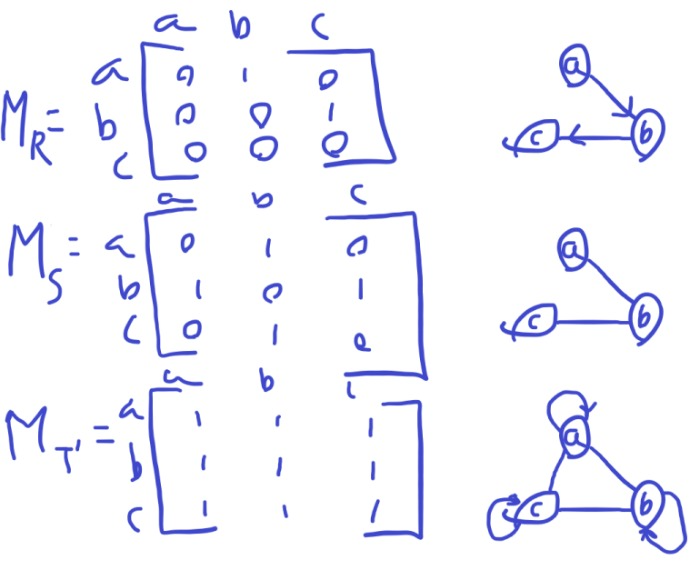
\includegraphics[width=0.75\textwidth]{img1.png}
    \caption{}
\end{figure}

Lad os nu gøre det samme, men vi tager transitivity først:
\[R=\{(a,b),(b,c)\}\]
\[transitivity\]
\[T=\{(a,b),(a,c),(b,c)\}\]
\[symmetri\]
\[S'=\{(a,b),(a,c),(b,a),(b,c),(c,a),(c,b)\}\]

\begin{figure}[H]
    \centering
    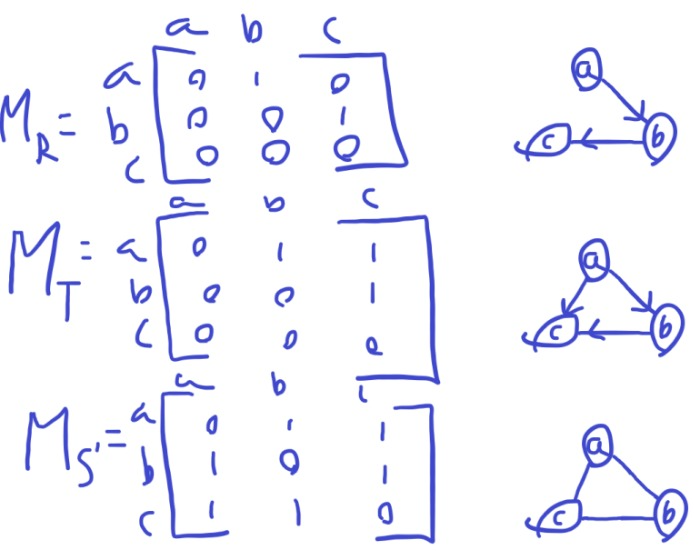
\includegraphics[width=0.75\textwidth]{img2.png}
    \caption{}
\end{figure}

Det er altså ikke altid tilfældet, at $S'$ og $T$ vil være ens, hvis vi tager den symmetric closure før den transitive closure.


\section[Question 5]{Recall that an undirected graph $G = (V, E)$ consists of a set of vertices $V$ connected by
edges $E$, where every edge is an unordered pair of vertices. If there is an edge $(u, v)$ between two
vertices $u$ and $v$, then we say that $u$ and $v$ are the endpoints of the edge, and the two vertices are
said to be neighbours. We say that a sequence of edges $(v_1, v_2), (v_2, v_3), (v_3, v_4), \ldots, (v_{k-1}, v_k)$,
in $E$ is a path from $v_1$ to $v_k$. In this problem, we wish to express properties of graphs in both natural language and pred-
icate logic, and to translate between the two forms. We do this as follows:
\begin{itemize}
\item The universe is the set of vertices $V$ of $G$.
\item The binary predicate $E(u, v)$ holds if and only if there is an edge between $u$ and $v$ in $G$.
\item The unary predicate $S(v)$ is used to identify a subset of vertices $S = \{v \mid v \in V, S(v) \text{ is true}\}$
for which some property might or might not hold.
\end{itemize}
For example, we can write the natural language statement "$S$ is a set containing exactly $k$ distinct
elements" as a formula
\[\text{setsize}(S, k) := \exists u_1 \cdots \exists u_k \left(\bigwedge_{i=1}^{k-1} \bigwedge_{j=i+1}^{k} (u_i \neq u_j) \wedge \bigwedge_{i=1}^{k} S(u_i) \right)\]
\[\wedge \neg \exists u_1 \cdots \exists u_{k+1} \left(\bigwedge_{i=1}^{k} \bigwedge_{j=i+1}^{k+1} (u_i \neq u_j) \wedge \bigwedge_{i=1}^{k} S(u_i) \right) \tag{1}\]
where $\bigwedge_{i=1}^{k} \phi_i$ is shorthand for $\phi_1 \wedge \phi_2 \wedge \cdots \wedge \phi_k$, and where we use standard notation $\neg$ for
logical negation. In natural language, this formula can be read as: "There exist $k$ elements $u_1$ to
$u_k$ such that (i) for every pair $(u_i, u_j), i \neq j$, the elements themselves are also distinct $(u_i \neq u_j)$;
and (ii) all the $u_i$ for $i = 1, \ldots, k$ are members of $S$, but no such set of $k+1$ elements $u_1$ to $u_{k+1}$
exists."
Below you find six graph properties defined in natural language and six graph properties
written as predicate logic formulas. Most of the natural language definitions have equivalent
predicate logic formulas, but not all.
Your task is to translate each predicate logic formula (a), $\ldots$, (f) into a natural language
description, and argue which—if any—of the natural language definitions (1), $\ldots$, (6) it matches.\\
\n
\textbf{Natural Language Definitions:}\\
\n
(1) A \emph{dominating set} of size $k$ for a graph $G = (V, E)$ is a set $S$ of $k$ distinct vertices such that every vertex $v$ in the graph either is in $S$ or is a neighbour of a vertex in $S$.\\
\n
(2) A \emph{clique} $S$ of size $k$ in a graph $G = (V, E)$ is a set $S$ of $k$ distinct vertices such that all vertices in $S$ are neighbours with each other.\\
\n
(3) A \emph{disconnected vertex set} of size $k$ in a graph $G = (V, E)$ is a set $S$ of $k$ distinct vertices such that there are no edges from any $u \in S$ to any $v \in V \setminus S$. [Here $V \setminus S$ denotes set subtraction, so that $V \setminus S = \{v \mid v \in V \text{ and } v \not\in S\}$.]\\
\n
(4) A \emph{vertex cover} of size $k$ of a graph $G = (V, E)$ is a set $S$ of $k$ distinct vertices such that for every edge $(u, v) \in E$ it holds that at least one of the endpoints is in $S$.\\
\n
(5) A graph $G = (V, E)$ is \emph{bipartite}, with one of the parts in the bipartition having size $k$, if there a set $S$ of $k$ distinct vertices such that all edges in the graph go between $S$ and $V \setminus S$.\\
\n
(6) A \emph{connected component} $S$ of size $k$ in a graph $G = (V, E)$ is a set $S$ of $k$ distinct vertices such that for every pair of distinct vertices $u$ and $v$ in $S$ there is a path from $u$ to $v$ consisting of vertices in $S$.\\
\n
\textbf{Predicate Logic Formulas:}\\
\n
(a) $setsize(S, k) \wedge \forall v \forall w \left(E(v, w) \rightarrow S(v) \vee S(w)\right)$\\
\n
(b) $setsize(S, k) \wedge \forall v \left(S(v) \vee \exists w(S(w) \wedge E(v, w))\right)$\\
\n
(c) $setsize(S, k) \wedge \forall u \forall w\left((u \neq w \wedge S(u) \wedge S(w)) \rightarrow \exists v(E(u, v) \wedge E(v, w))\right)$\\
\n
(d) $setsize(S, k) \wedge \forall v \forall w\left(E(v, w) \rightarrow ((S(v) \wedge \neg S(w)) \vee (\neg S(v) \wedge S(w)))\right)$\\
\n
(e) $setsize(S, k) \wedge \forall v\left(S(v) \rightarrow \exists w(\neg S(w) \wedge E(v, w))\right)$\\
\n
(f) $setsize(S, k) \wedge \forall v \forall w\left((v \neq w \wedge S(v) \wedge S(w)) \rightarrow E(v, w)\right)$\\
\n
For every predicate logic formula that matches a natural language description, explain clearly why there is a match. For formulas that do not match a description, write a natural language definition along the lines of (1), \ldots, (6) that describes the property that the formula encodes.}


\subsection{Oversættelse af Predicate Logic Formulas}
Jeg vælger at oversætte alle formlerne først, hvorefter vi finder den bedst passende beskrivelse til dem.\\

(a) Et sæt $S$ af en graf $G=(V,E)$ bestående af $k$ unikke vertices, hvor alle de vetices der har en edge er med i $S$.\\

(b) Et sæt $S$ af en graf $G=(V,E)$ bestående af $k$ unikke vertices, hvor enhver vertex i grafen enten selv er i $S$ eller er nabo til mindst en vertex i $S$.\\

(c) Et sæt $S$ af en graf $G=(V,E)$ bestående af $k$ unikke vertices, hvor for ethvert par af forskellige vertices $u,w \in S$ findes der en vertex $v$ i grafen, som er forbundet direkte til både $u$ og $w$.\\

(d) Et sæt $S$ af en graf $G=(V,E)$ bestående af $k$ unikke vertices, hvor for enhver edge $(v,w) \in E$ gælder det, at præcis et af vertices'ne er i $S$ (altså enten $v \in S$ og $w \notin S$, eller $v \notin S$ og $w \in S$). Dette beskriver en bipartition graf, hvor $S$ udgør den ene del af opdelingen.\\

(e) Et sæt $S$ af en graf $G=(V,E)$ bestående af $k$ unikke vertices, hvor enhver vertex $v \in S$ har mindst en edge med en vertex $w$ som ikke er i $S$.\\

(f) Et sæt $S$ af en graf $G=(V,E)$ bestående af $k$ unikke vertices, hvor alle vetices har en edge med en vertex, som ikke er sig selv.\\

\subsection{Matching af Natural Language Definitions}
(a) Dette beskriver et sæt $S$ af størrelse $k$, hvor for enhver edge $E(v,w)$ er mindst et af endepunkterne $v$ eller $w$ i $S$. Dette svarer præcis til definition ($4$) for et vertex cover.\\
\\
(b) Dette beskriver et sæt $S$ af størrelse $k$, hvor enhver vertex $v$ enten selv er i $S$ eller har en nabo $w$ der er i $S$. Dette svarer til definition (1) for et dominating set.\\
\\
(c) Dette beskriver, at for ethvert par af forskellige vertices $u$,$w$ i $S$ findes der en vertex $v$, som er forbundet direkte til både $u$ og $w$. Dette matcher ikke direkte nogen af definitionerne.\\
\\
(d) Dette beskriver at for enhver edge $E(v,w)$ er præcis et af endepunkterne i $S$. Dette svarer til definition (5) for en bipartite graf.\\
\\
(e) Dette beskriver at enhver vertex $v$ i $S$ har mindst en edge til en vertex $w$ som ikke er i $S$. Dette matcher ikke direkte nogen af definitionerne.\\
\\
(f) Dette beskriver at for ethvert par af forskellige vertices $v$,$w$ i $S$, er de forbundet med en edge. Dette svarer til definition (2) for en clique.\\

\end{document}